
\section{Performance test}
\label{sec:perf}

\begin{frame}
    \frametitle{Google Benchmark}
    \begin{table}
        \centering
    \begin{tabular}{|c|c|c|c|}
        \toprule
        Benchmark/\#Particles & Time & CPU & Iterations \\
        \toprule
        BM\_LJSimulation/1000 & 1.4485e+10 ns & 1.4477e+10 ns & 1 \\
        \midrule
        BM\_LJSimulation/2000 & 5.7983e+10 ns & 5.7959e+10 ns & 1 \\
        \midrule
        BM\_LJSimulation/4000 & 2.3180e+11 ns & 2.3171e+11 ns & 1 \\
        \midrule
        BM\_LJSimulation/8000 & 9.2722e+11 ns & 9.2686e+11 ns & 1 \\
        \midrule
        BM\_LJSimulation\_BigO & 14487.81 $N^2$ & 14482.20 $N^2$ & - \\
        \midrule
        BM\_LinkedLJSimulation/1000 & 28515871 ns & 28493193 ns & 25 \\
        \midrule
        BM\_LinkedLJSimulation/2000 & 54951418 ns & 54934137 ns & 13 \\
        \midrule
        BM\_LinkedLJSimulation/4000 & 114455900 ns & 114424760 ns & 6 \\
        \midrule
        BM\_LinkedLJSimulation/8000 & 236827726 ns & 236733811 ns & 3 \\
        \midrule
        BM\_LinkedLJSimulation\_BigO & 29304.28 $N$ & 29293.31 $N$ & - \\
        \bottomrule
    \end{tabular}
    \end{table}
\end{frame}

\begin{frame}
    \frametitle{Graphs}
    \textbf{Results show improvement from squared to linear runtime!}
    \begin{figure}
        \label{fig:timelc}
        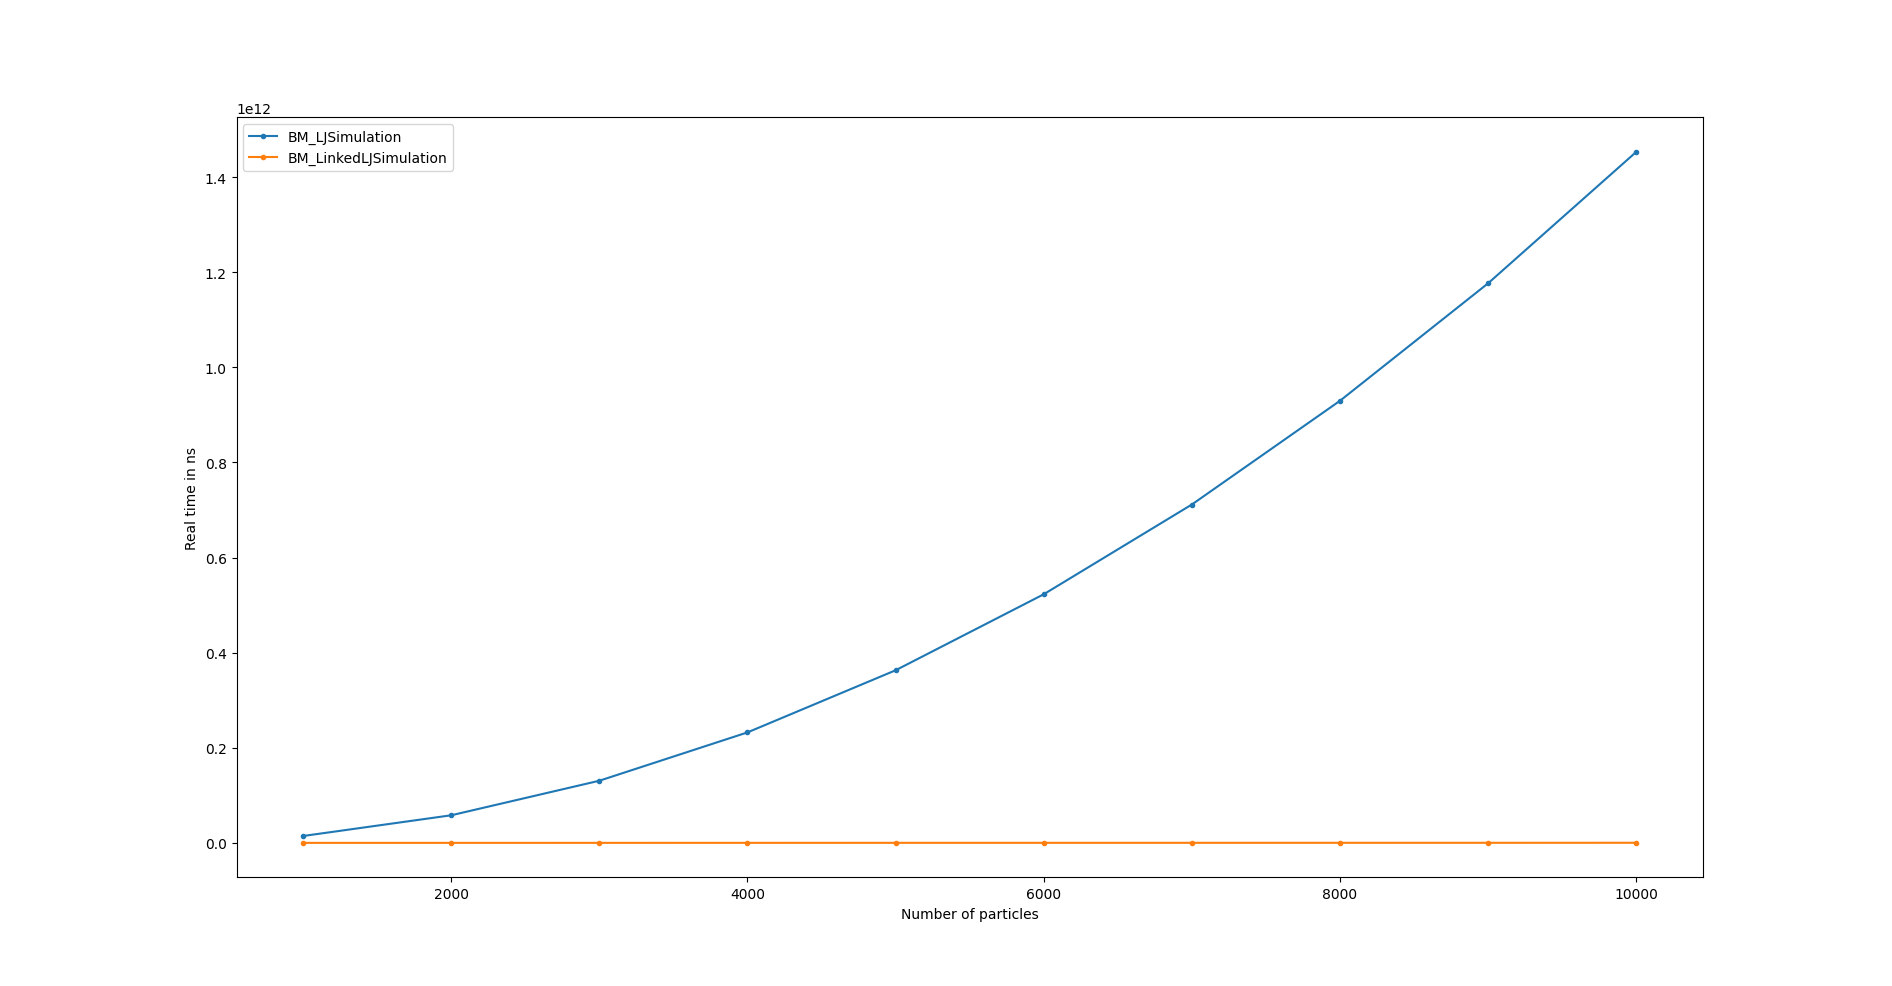
\includegraphics[width=0.9\textwidth]{../../res/lj_big_plot_linear}
    \end{figure}
\end{frame}

\begin{frame}
    \frametitle{Graphs}
    \begin{figure}
        \label{fig:timelclog}
        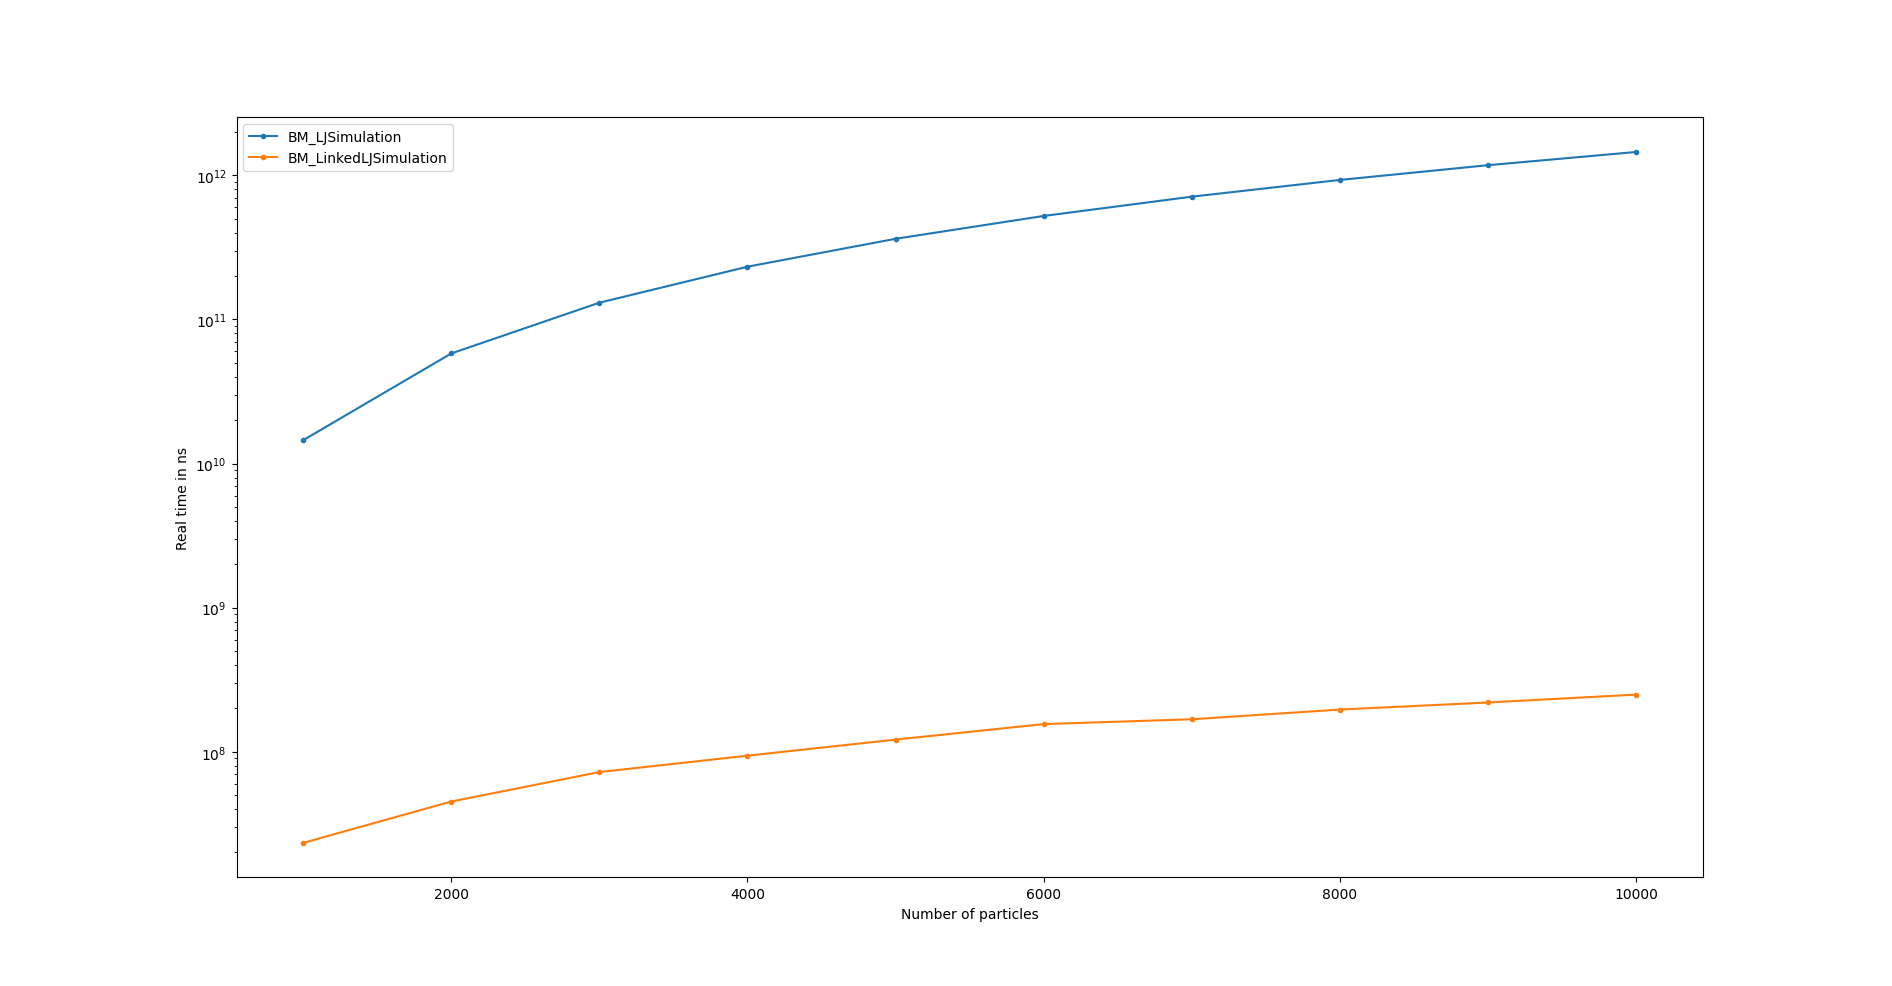
\includegraphics[width=0.9\textwidth]{../../res/lj_big_plot_log}
    \end{figure}
\end{frame}
